\subsubsection{Bình luận và rating cho nhà}
\subsubsubsection{User Story}
\textit{Diamond Stay} sẽ cho phép người dùng ứng dụng bình luận và rating cho nhà. Đây là một chức năng sẽ giúp người dùng có thể nêu lên quan điểm, đánh giá của mình về nhà. Từ đó, sẽ giúp cho người dùng khác tham khảo khi chọn lựa nhà trên hệ thống.
\subsubsubsection{Mô tả các use case}
\begin{enumerate}[label=\textbf{(\alph*)}]
    \begin{figure}[!h]
    	\centering
    	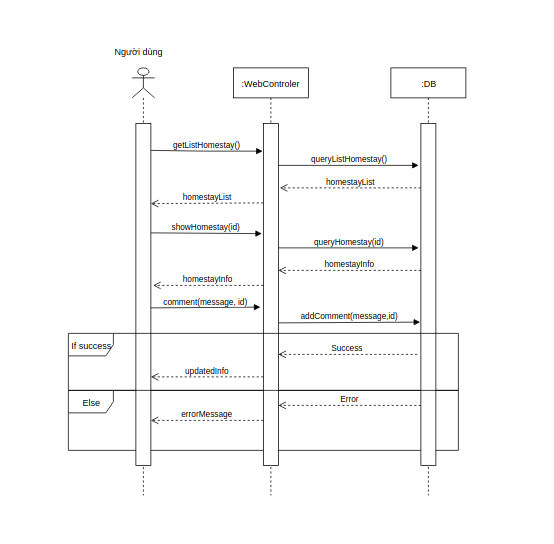
\includegraphics[width=13cm]{Image/tin-sequence-comment.png}
    	\caption{Sequence Diagram cho usecase bình luận}
    \end{figure}
	\item \textbf{Usecase 1: Bình luận cho nhà.}
	\begin{center}
		\begin{longtable}{ | l |p{10cm}|}
			\hline
			\textbf{Tên usecase} & Bình luận cho nhà \\ \hline
			\textbf{Người tương tác} & Người dùng ứng dụng \\ \hline   
			\textbf{Mô tả} &  Cho phép người dùng ứng dụng bình luận đối với nhà.\\ \hline  
			\textbf{Người tạo:} \textit{Trần Ngọc Tín} & \textbf{Cập nhật lần cuối bởi:} \textit{Trần Ngọc Tín} \\ \hline
			\textbf{Ngày tạo:} \textit{22/03/2019} & \textbf{Lần cuối cập nhật:} \textit{30/03/2019} \\ \hline
			\textbf{Tiền điều kiện} &  Người dùng phải đăng nhập vào hệ thống. \\ \hline 
			\textbf{Hậu điều kiện} &  Nhà được người dùng bình luận. \\ \hline 
			\textbf{Luồng cơ bản} & 
			\begin{enumerate}
			\item Người dùng chọn tab tìm nhà (có thể áp dụng bộ lọc)
    \item Hệ thống hiển thị danh sách nhà theo bộ lọc và rating có sẵn
    \item Người dùng click vào nhà muốn bình luận
    \item Hệ thống hiển thị thông tin chi tiết của nhà, trong đó có các bình luận hiện tại của nhà đó
    \item Người dùng điền bình luận của mình vào ô thêm bình luận và nhất nút "Thêm"
    \item Bình luận của người dùng được cập nhật trong thông tin nhà
			\end{enumerate} \\ \hline 
			\textbf{Luồng thay thế} & 
			\begin{enumerate}
				\item Tại bước 6: Nếu xảy ra lỗi trong khi thêm bình luận
				\item Hệ thống báo lỗi ra cho người dùng
			\end{enumerate} \\ \hline
		
			\textbf{Ngoại lệ}  & Không có \\
			\hline
		\end{longtable}
	\end{center}
	\newpage
	\begin{figure}[!h]
        	\centering
        	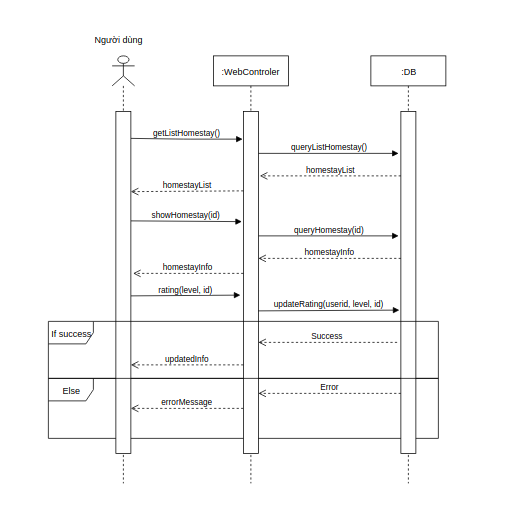
\includegraphics[width=13cm]{Image/tin-sequence-rating.png}
        	\caption{Sequence Diagram cho usecase rating homestay}
    \end{figure}
		\item \textbf{Usecase 2: Rating cho nhà.}
	\begin{center}
		\begin{longtable}{ | l |p{10cm}|}
			\hline
			\textbf{Tên usecase} & Rating cho nhà \\ \hline
			\textbf{Người tương tác} & Người dùng ứng dụng \\ \hline   
			\textbf{Mô tả} &  Cho phép người dùng ứng dụng rating đối với nhà.\\ \hline  
			\textbf{Người tạo:} \textit{Trần Ngọc Tín} & \textbf{Cập nhật lần cuối bởi:} \textit{Trần Ngọc Tín} \\ \hline
			\textbf{Ngày tạo:} \textit{22/03/2019} & \textbf{Lần cuối cập nhật:} \textit{30/03/2019} \\ \hline
			\textbf{Tiền điều kiện} &  Người dùng phải đăng nhập vào hệ thống. \\ \hline 
			\textbf{Hậu điều kiện} &  Nhà được người dùng rating. \\ \hline 
			\textbf{Luồng cơ bản} & 
			\begin{enumerate}
		\item Người dùng chọn tab tìm nhà (có thể áp dụng bộ lọc)
        \item Hệ thống hiển thị danh sách nhà theo bộ lọc và rating có sẵn
        \item Người dùng click vào nhà muốn rating
        \item Hệ thống hiển thị thông tin chi tiết của nhà, trong đó có rating hiện tại của nhà đó
        \item Người dùng click vào mức rating từ 1 đến 5 sao
        \item Rating của người dùng được cập nhật trong thông tin nhà
			\end{enumerate} \\ \hline 
			\textbf{Luồng thay thế} &
				\begin{enumerate}
    				\item Tại bước 6: Nếu xảy ra lỗi trong khi rating
    				\item Hệ thống báo lỗi ra cho người dùng
    			\end{enumerate} \\ \hline
			\textbf{Ngoại lệ}  & Không có \\
			\hline
		\end{longtable}
	\end{center}
\end{enumerate}